%% RT-plots-new.tex
%% Images from the new Radon output 

\begin{figure*}
    \centering
    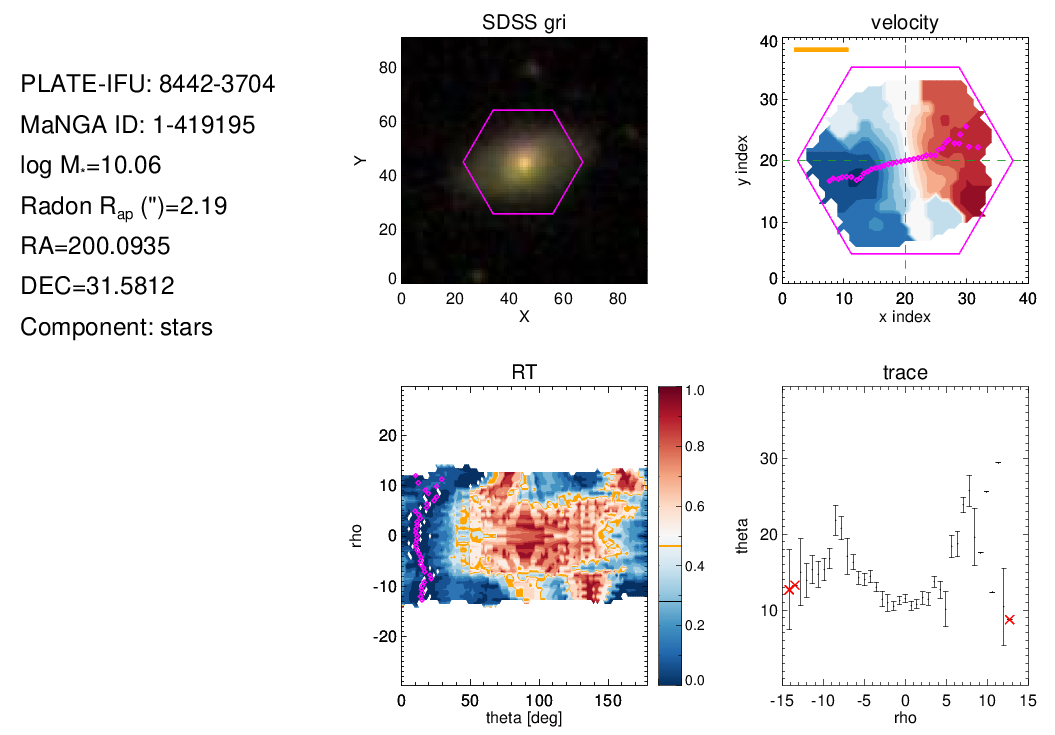
\includegraphics[width=0.9\textwidth]{images/RadonPlots/RT-SNIPS-NEW/8442-3704-complete.png}
    \caption[Radon transform code output graphics for stellar velocity field of the MaNGA plateifu 8442-3704]{The Absolute Radon transform code output graphics for the stellar velocity field of the galaxy MaNGA plateifu 8442-3704. The left side text block provides some relevant data about the galaxy extracted from the MaNGA DAP. The quadrature arrangement of panels to the right show: top left - the SDSS IFU gri image cutout; top right - the stellar velocity field with kinematic position angle PA\k superimposed by the magenta line. The orange coloured  bar in the upper left indicates the Radon aperture size in spaxels; bottom left - the absolute value of Radon transform re-scaled from 0 to 1. The locus of the minimum of the transform is plotted in magenta; and bottom right: the Radon trace plot.}
    \label{fig:8442-3704-complete}
\end{figure*}

This Radon transform code output for this particular galaxy, MaNGA ID 1-419195 plateifu 8442-3704, reveals some particularly significant stellar kinematic features, however at this point we have not classified the galaxy in terms of its Radon profile type. Radon profile classification will be discussed in some depth in Section \ref{sec:Radon-classification}. 